\documentclass[../dissertation.tex]{subfiles}

\begin{document}

% Middlewares mentioned:
% CORBA, Player, OpenRDK, ROS, MOOS

Middleware designs can be broken down in to four groups of concepts: Communication, Computation, Configuration, and Coordination \cite{brugali2010component}. The majority of robotic middleware differences can be demonstrated as a difference in one of these groups. The following sections provide an overview of the approaches that the middlewares summarised above use to tackle each of these areas.

\subsection{Communication}

All modern robotic middlewares are comprised of multiple modules. In a non-trivial robotic system these distinct modules must exchange a variety of information in a complex web. These information channels usually have some desired bounds or characteristics, such as reliability (guarantees on information delivery), performance (general low latency, or some guarantees on delivery times), and overhead (is the communication significantly more expensive than building one monolithic module). The middlewares presented in Section \ref{overview-of-robotic-middleware} have used a variety of approaches to inter-component communication.

CORBA, and those middlewares built on top of CORBA utilise a remote object abstraction. This allows for inter-component communication to appear consistent whether the method caller and callee exists in the same address space, or in a remote address. The only explicit step to enable remote object communication is to share the object reference with the remote process (or component). This is achieved via an Object Request Broker (ORB), which objects can be registered with, and references retrieved from. This form of communication provides very neat code abstractions (as there is no need to modify how the object is used, only how the reference is acquired).

\begin{figure}[H]
\centering
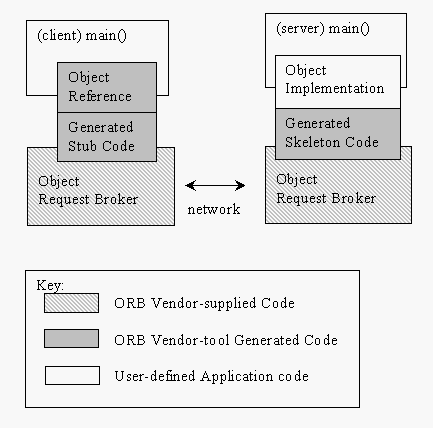
\includegraphics[width=0.5\textwidth]{images/background/Orb.png}
\caption{Illustration of the communication infrastructure when using CORBA\cite{corbaCommunicationWikipediaImage}.}
\end{figure}

Other middlewares such as ROS have a more explicit communication paradigm. ROS uses a network of software nodes which can create message queues (known as a topic), which they can publish data of a specific type to \cite{rosconcepts}. Other nodes can subscribe to topics, generally registering a callback function which is called when some new data has been published to the topic. These mechanisms are described in detail in Section \ref{background-ros}. This method of communication also allows for code to be identical whether or not the two communicating nodes are in the same address space or are remote, but the communication code itself is explicit. The programmer must define when the topics are created, when data is published, and what happens in a subscriber when the data is published.

\begin{figure}[H]
\centering
\includegraphics[width=0.5\textwidth]{images/background/ROS_Explained.png}
\caption{ROS node communication}
\end{figure}

OpenRDK utilises a blackboard model. The analogy refers to the idea of many people stood around a blackboard and communicating only via writing things in different areas of the blackboard, without direct communication between the individuals. This is a form of centralised communication. In OpenRDK the blackboard is called a repository, and each module can communicate by publishing values (called properties) to the repository \cite{OpenRDKIntro}. Properties can be simple values, or a queue object. The properties are addressed via a global hierarchical URL-like addressing scheme, similar to ROS topic addressing.

Player consists of a centralised server which connects to control clients via a standard TCP socket \cite{PlayerServerManual}. The client and server communicate via a set of simple messages. This is a lower-level communication paradigm which is very explicit in code, and requires careful control of shared resources as very little is provided by the library.

\subsection{Computation}

Each module created using a robotic middleware is generally tasked with some computation. That computation could be as simple as processing a value read from a sensor, and publishing it to some communication channel, or as complex as a multi-layered object classifier for images requiring large amounts of computation. Middlewares need to support these use-cases and everything in between, with a coherent, consistent infrastructure model. Middlewares generally provide a way of decoupling distinct computational tasks so that they can be individually designed, implemented, and tested - and then coupled together using the middleware's communication and coordination framework.

OpenRDK models computation inside modules \cite{OpenRDKIntro}. Each module runs on a single thread, and multiple modules are grouped together to form an agent (a single process).

ROS has a less layered system. Computations are performed by nodes and these nodes directly communicate with each other. Each node generally performs a single focused task. A node usually consists of a single thread, but the programmer is free to spawn new threads as they require. See Section \ref{background-ros} for a more complete description of ROS.

All of the presented middlewares present a similar computation structure as the previous two examples, if they prescribe a computation structure at all. For example, CORBA says nothing about how the robotic application is structured, merely that object references must be shared via the Object Request Broker.

\subsection{Configuration}

The configuration of a robotic system using a middleware is often specified using some mechanic of the middleware. There are several distinct stages at which configuration is important, such as compile-time, deployment-time, and run-time. Compile-time configuration involves specifying what compiler settings are required, what libraries should be linked to (and their versions), and what structures and metadata should be created. Configuration at deployment-time involves setting up the system the robotic software is running on - such as installing libraries via a package manager, copying software to specific locations, and setting environment variables. Run-time configuration has a wide variety of potential uses, but can consist of specifying API keys, database connection details, the number of threads that should be created for each process, the particular modules that should start (and when they should start), how components should interconnect and communicate with each other, and how exceptions should be handled.

ROS uses XML files at compile-time to resolve dependencies, export version numbers, and other miscellaneous meta information such as software license and author details. The ability to define the launch of ROS nodes is provided by the `roslaunch' package. This package parses an XML file which defines which nodes should run, and also sets any required parameters on the ROS Parameter Server. It also provides some reliability functionality, such as respawning processes that have died \cite{roslaunchPage}. ROS includes another way for new agents (nodes) to configure themselves - in the form of a parameter server. This parameter server runs on the ROS master node, providing a central repository of settings. New non-master nodes can request specific parameters from this server at deployment-time (and run-time). This means that configuration files need not be modified in all running instances of the nodes, merely the information stored by the master node need be modified - providing a more centralised configuration than simple local files.

MOOS also utilises a text file for runtime configuration called a `Mission file' \cite{newman2009introduction}. This mission file provides the necessary runtime parameters for components to set themselves up in a system. However, this configuration is simpler than ROS' systems - primarily it functions as a key-value store for MOOS processes.

OpenRDK utilises an XML configuration file to do similar tasks. However it is closer to ROS in terms of flexibility than MOOS, providing advanced key-value store mechanics, as well as a `yellow pages' - a lookup table to contact the various agents running in the system.

\subsection{Coordination}

Most middlewares have explicit mechanisms for creating multiple concurrently running software components. These components need to exhibit some overall system behaviour, usually by working together. It is not enough for each component to independently run and share data, there needs to be some coordination to the system to provide controlled, reliable, behaviour. For this reason, some middlewares provide concurrency libraries, either explicitly, or implicitly such as by the computation and communication model or by language features.

In ROS, this concurrency is managed by running all nodes in separate threads, and designing the nodes in a reactive model. The node's computation only occurs when there is data to process, or some task to complete. In this model, subscribers to a particular data stream are immediately aware of when new data has been published and can begin processing immediately - reducing processing latencies.

OpenRDK agents communicate with each other primarily via the repository (a blackboard-type object). This simplifies the communication model of OpenRDK processes, but limits the behaviour of each client to only a pull-type of communication, meaning that each client must individually check the repository to see if there's new data to process. Each producer of data must wait for it's clients to check the blackboard, as it cannot directly tell the client to process new data.

Interconnections between components in many middlewares are achieved over TCP connections with the middleware libraries handling (de)serialization of the messages. Some middlewares such as Player are designed for a client/server architecture, with no/little intercommunication between client components, whereas ROS is designed entirely as a direct P2P network topology (with the master node mainly providing address look-up).

\end{document}
